\documentclass{article}
\usepackage{graphicx} % Required for inserting images


\begin{document}

Optica geometrica
Area de la fisica que estudia la naturaleza de la luz y sus interacciones
En optica geometrica estudiamos "trayectorias" que sigue la luz al propagarse c \approx 3 \cdot 10^8ms^{-1}

Principio de Fermat 150a.c. - 250d.c Hero de alejandria
"La trayectoria tomada por al luz para ir de un punto S a un punto P a traves de una superficie reflectora es la mas corta posible.
\begin{figure}
    \centering
    
\includegraphics[width=0.5\linewidth]{image.png}
    \label{fig:placeholder}
\end{figure}

La trayectoria mas corta es \theta_i = \theta_r

1657
Fermat propone "principio del tiempo minimo", "la trayectoria real que adopta un haz de luz entre dos puntos es aquella recorrida en el menor tiempo"

\begin{figure}
    \centering
    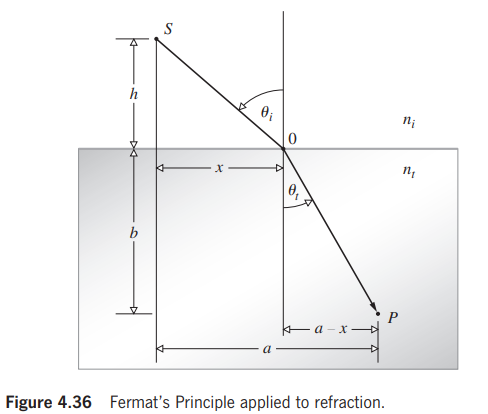
\includegraphics[width=0.75\linewidth]{Fermat’s Principle applied to refraction.png}
    \caption{Fermat’s Principle applied to refraction.}
    \label{fig:placeholder}
\end{figure}

 \[
\begin{array}{c}
t=\frac{\overline{S O}}{v_{i}}+\frac{\overline{O P}}{v_{t}} \\
\text { or } \quad t=\frac{\left(h^{2}+x^{2}\right)^{1 / 2}}{v_{i}}+\frac{\left[b^{2}+(a-x)^{2}\right]^{1 / 2}}{v_{t}}
\end{array}
\]

To minimize \( t(x) \) with respect to variations in \( x \), we set \( d t / d x=0 \), that is,
\[
\frac{d t}{d x}=\frac{x}{v_{i}\left(h^{2}+x^{2}\right)^{1 / 2}}+\frac{-(a-x)}{v_{t}\left[b^{2}+(a-x)^{2}\right]^{1 / 2}}=0
\]

Using the diagram, we can rewrite the expression as
\[
\frac{\sin \theta_{i}}{v_{i}}=\frac{\sin \theta_{t}}{v_{t}}
\]
which is no less than Snell's Law (Eq. 4.4). If a beam of light is



\end{document}
